    \documentclass{article}
\usepackage{graphicx} % Required for inserting images
\usepackage{titling}
\usepackage{enumitem} % Per personalizzare elenchi puntati
\usepackage{hyperref}
\usepackage{amsmath}
\usepackage{multirow}
\usepackage{etoolbox}

\renewcommand{\contentsname}{Indice}

\begin{document}

\begin{title}
    \centering
    \huge\bfseries  % Grandezza e grassetto per il titolo
    \noindent
    Fisica
\end{title}
\vspace{60pt}
\tableofcontents

\newpage

\section{Cinematica}
La \textit{cinematica} fornisce le metodologie fondamentali per analizzare il moto, utilizzando due concetti chiave: la velocità e l'accelerazione.
\subsection{Equazione del moto}
L'\textit{equazione del moto} è rappresentata dalla funzione \(x(t)\), che esprime la posizione \(x\) in funzione del tempo \(t\).
\subsection{Velocità}
La \textit{velocità media} è definita come il rapporto tra la variazione di posizione \(\Delta x\) e la variazione di tempo \(\Delta t\), ottenute come:
\[\Delta x = x_2 - x_1\]
\[\Delta t = t_2 - t_1\]
Il rapporto tra queste grandezze è dato da:
\[
v_m = \frac{\Delta x}{\Delta t} = [\frac{m}{s}]
\]
Dal punto di vista grafico, questo può essere rappresentato come segue:
\begin{figure}[ht]
    \centering
    \includegraphics[width=0.61\linewidth]{Immagini/Velocità Media.png}
    \caption{Velocità Media}
\end{figure}
\\
\noindent Scomponendo il grafico e riducendo \(\Delta t\) a \(0\), possiamo definire la \textit{velocità istantanea} come:
\[
v(t) = \lim_{\Delta t\to 0} \frac{\Delta x}{\Delta t} = \frac{dx}{dt}
\]
\\
Questa è anche rappresentata dalla derivata dell'equazione del moto.\\
\\
Possiamo ora definire l'equazione per calcolare la posizione dato un certo valore di velocità\\
\\
\textbf{Moto uniforme}:
\[
x(t) = x_0 + v_1 (t_1 - t_0)
\]
\subsection{Accelerazione}
L'accelerazione rappresenta la variazione della velocità rispetto al tempo. Possiamo definire l'\textit{accelerazione media}, relativa all'intervallo di tempo \(\Delta t = t_2 - t_1\), come il rapporto:
\[
    a_m = \frac{v_2 - v_1}{t_2 - t_1} =\frac{\Delta v}{\Delta t} = [\frac{m}{s^2}]
\]

\noindent Anche in questo caso è possibile, riducendo al minimo il valore \(\Delta t\), trovare il valore di accelerazione istantanea.
Questo come
\[
a(t)= \lim_{\Delta t\to 0} \frac{\Delta v}{\Delta t} = \frac{dv}{dt} = \frac{d^2x}{dt^2}
\]
Dal punto di vista grafico, questo può essere rappresentato come segue:
\begin{figure}[ht]
    \centering
    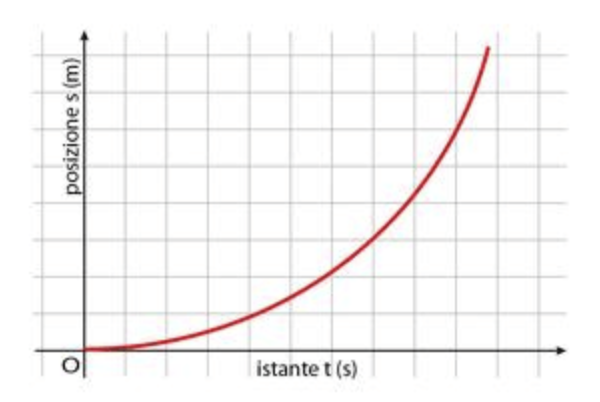
\includegraphics[width=0.75\linewidth]{Immagini/Accelerazione Spazio-Tempo.png}
    \caption{Accelerazione Spazio-Tempo}
\end{figure}
\newpage
\noindent Da qui è possibile ottenere le principali formule del \\
\\
\textbf{Moto uniformemente accelerato}
\[
v = v_0 + a \cdot t
\]
\[
s = s_0 + v_0t + \frac{1}{2}at^2
\]
\[
s = \frac{v^2 - v^2_0}{2a}
\]
\textbf{Moto uniformemente decelerato}
\[
v = v_0 - a \cdot t
\]
\[
s = s_0 +v_0t - \frac{1}{2}at^2
\]
\[
s = \frac{v^2_0 - v^2}{2a}
\]
\subsection{Moto Parabolico}
Il moto parabolico è il movimento di un oggetto lanciato in un campo gravitazionale, dove la traiettoria descrive una parabola. Le equazioni che descrivono la posizione dell'oggetto in funzione del tempo sono:
\[
\begin{cases}
    x = v_0 cos \theta \cdot t \\
    y = y_0 + v_0 sin \theta \cdot t - \frac{1}{2}g t^2
\end{cases}
\]
\\
\textbf{Gittata (Distanza asse x)}\\
La gittata è la distanza orizzontale totale percorsa dall'oggetto. Può essere calcolata con la seguente formula:
\[
    G = \frac{2\cdot v_0 cos(\theta) \cdot v_0 sin(\theta)}{g}
\]
\\
\textbf{Gittata massima (con angolo 45°)}\\
La gittata massima si ottiene quando l'angolo di lancio è di 45°. In questo caso, la formula semplificata per la gittata massima è:
\[
    G = \frac{(v_0)^2}{g}
\]
\\
\textbf{Altezza massima (h asse y)}\\
L'altezza massima raggiunta dall'oggetto può essere determinata con la seguente formula:
\[
    h = \frac{(v_0 \cdot sin(\theta))^2}{2 \cdot g}
\]
\\
\textbf{Tempo in volo}\\
Il tempo totale di volo è il tempo che l'oggetto impiega per tornare al livello di partenza, e può essere calcolato con:
\[
    t = \frac{2 \cdot v_0 sin(\theta)}{g}
\]
\subsection{Moto circolare}
\subsubsection{Moto circolare uniforme}
Il moto circolare uniforme è il moto in cui un corpo si muove lungo una traiettoria circolare con velocità tangenziale \(\Vec{v}\) costante.
\begin{figure}[ht]
    \centering
    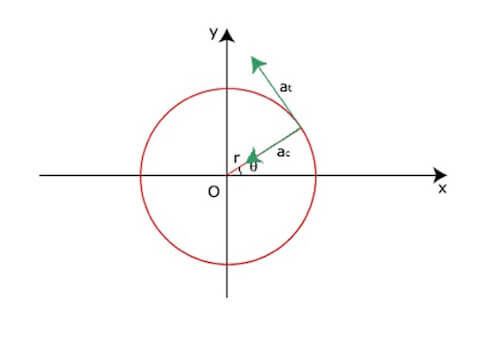
\includegraphics[width=0.7\linewidth]{Immagini/circolare.png}
\end{figure}
\noindent\textbf{Velocità tangenziale}
\[
\Vec{v} = \frac{s}{t} = \frac{2\pi r}{T}
\]
oppure
\[
\Vec{v} = \omega r
\]
dove \(2\pi r\) è la circonferenza e \(T\) è il periodo.
\\
\\
\textbf{Velocità angolare}\\
La velocità angolare è la velocità con cui il punto materiale si muove lungo la circonferenza.
\[
    \Vec{\omega} = \frac{2 \pi}{T} 
\]
\newpage
\noindent \textbf{Frequenza}
\[
    f = \frac{1}{T} = [Hz]
\]
\textbf{Accelerazione centripeta}\\
L'accelerazione centripeta è l'accelerazione tale per cui la velocità tangenziale cambia direzione.
\[
    \Vec{a}_c = \frac{v^2}{r} = \omega^2r
\]
\subsubsection{Moto circolare uniformemente accelerato}
Il moto circolare uniformemente accelerato è il moto in cui un corpo, in movimento lungo la traiettoria circolare, è sottoposto ad un'accelerazione tangenziale costante.\\
\\
\textbf{Accelerazione totale}
\[
    \Vec{a}_{tot} = \Vec{a}_T + a_c
\]
oppure
\[
    \left|\Vec{a}_{tot}\right| = \sqrt{a_T^2 +a_c^2}
\]
\\
\textbf{Accelerazione tangenziale}
\[
    \left|\Vec{a}_{T} \right| = \alpha r,
\]
dove    
\[
    \alpha = \frac{\Delta \omega}{\Delta t}
\]
\\
\textbf{Legge oraria}\\
La legge oraria esprime la variazione dell'angolo in funzione del tempo \(t\):
\[
    \Theta(t) = \frac{1}{2}at^2 + \omega_0t + \Theta_0
\]
\\
\textbf{Velocità angolare}\\
La velocità angolare in funzione del tempo \(t\) è:
\[
    \omega(t) = \omega_0 + \alpha t
\]
\newpage
\subsection{Moto armonico}
Il moto armonico è la proiezione lungo una retta (il diametro) di un punto che si muove in moto circolare uniforme. Nella figura, il punto verde rappresenta questa proiezione.
\begin{figure}[ht]
    \centering
    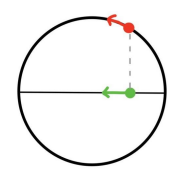
\includegraphics[width=0.3\linewidth]{Immagini/armonico.png}
\end{figure}

\noindent \textbf{Legge oraria}
\[
    x = r \cdot cos(\omega_0t + \phi)
\]
\noindent\textbf{Velocità}
\[
\Vec{v}= \frac{dx(t)}{dt} = -r \omega \sin(\omega_0t + \phi)    
\]
dove la velocità massima si ottiene quando \(sin(\omega_0t + \phi) = 1\):
\[
v_m = \omega r 
\]
\noindent\textbf{Accelerazione}
\[
\Vec{a} = \frac{dv(t)}{dt} = -r\omega^2 \cos(\omega_0t + \phi) = -\omega^2 x(t)
\]
dove l'accelerazione massima si ottiene quando \( \cos(\omega_0t + \phi) = 1\):
\[
a_m = -r\omega^2
\]
\subsection{Periodo di un pendolo}
Il periodo di un pendolo, rappresentato dalla variabile \( T \), è il tempo impiegato affinché il pendolo compia un'oscillazione completa da un'estremità all'altra e ritorni alla posizione di partenza. Questo periodo dipende dalla lunghezza del pendolo (\( l \)) e dall'accelerazione dovuta alla gravità (\( a \)).
\[
    T = 2\pi \cdot \sqrt{\frac{l}{a}}
\]
\newpage







\section{Dinamica}
La dinamica si basa su tre principi non dimostrabili
\begin{enumerate}
    \item Primo principio, o Principio d'inerzia
    \item Secondo principio (detto anche Legge fondamentale)
    \item Terzo principio (Principio di azione e reazione)
\end{enumerate}
\subsection{Il Primo principio( Principio d'inerzia)}
Il Primo Principio afferma:\textit{Un corpo non soggetto a forze permane in uno stato di quiete oppure di
moto rettilineo uniforme}.\\
\\
La tendenza dei corpi a mantenere inalterato lo stato di quiete o di moto rettilineo uniforme si
chiama \textit{inerzia}.
\subsection{Il secondo principio (legge fondamentale)}
L'enunciato del Secondo Principio può venire decomposto in una successione di affermazioni.
\begin{enumerate}
    \item L'effetto di una forza \(\Vec{F}\) applicata ad un corpo libero è un'accelerazione \(\Vec{a}\)  avente uguale
    direzione e verso della forza
    \item L'intensità dell'accelerazione di un corpo è proporzionale all'intensità della forza applicata.
    \item La medesima forza agente su corpi diversi provoca accelerazioni di modulo diverso, a causa
    della diversa \textit{inerzia} dei corpi. Quanto maggiore è l'inerzia, tanto minore è
    l'accelerazione. Per misurare l'inerzia di un corpo, si introduce una nuova grandezza, la massa
    m. A parità di forza agente su due corpi, vale la relazione \(m_1/m_2 = a_2/a_1\) (l'accelerazione è
    inversamente proporzionale alla massa).
    \item Poiché la forza ha carattere vettoriale, la risultante di più forze applicate contemporaneamente
    ad un corpo si calcola mediante la regola del parallelogramma.
\end{enumerate}
Questo viene riassunto in 
\[
\sum_{}^{i} \Vec{F_i} = m\Vec{a} = [N]
\]
dove \(\sum_{}^{i} \Vec{F_i}\) rappresenta la risultante delle forze applicate, \(m\) la massa e \(\Vec{a}\) l'accelerazione.
\subsection{Il terzo principio (Principio di azione e reazione)}
Il Terzo Principio afferma: \textit{Se un corpo A esercita una forza \(\Vec{F}_{AB}\) su di un corpo B, allora il corpo
B esercita sul corpo A una forza uguale e contraria \(\Vec{F}_{BA} = - \Vec{F}_{AB}\)}.

\subsection{Formula generica}
Nel caso in cui la forza non sia applicata in modo parallelo rispetto allo spostamento e vi sia anche un attrito dinamico possiamo trovare che
\[
\begin{cases}
  N = mg - F \cdot sen(\theta) \\
  F_{//} = F \cdot cos(\theta) - \mu N
\end{cases}
\]
Dove \(\theta\) rappresenta l'angolo di inclinazione della forma e \(\mu\) rappresenta il coefficiente di attrito dinamico.
\subsection{Forza Elastica legge di Hooke}
La forza centripeta è la forza che agisce su un corpo in movimento lungo una traiettoria circolare e che è diretta verso il centro del cerchio. Questa forza è necessaria per mantenere il corpo in un moto circolare. La formula per la forza centripeta \( F_c \) è data da:
\[
    \Vec{F}_e = - k\Vec{x}
\]
\subsection{Forza Centripeta}
La forza centripeta è la forza che agisce su un corpo in movimento lungo una traiettoria circolare e che è diretta verso il centro del cerchio. Questa forza è necessaria per mantenere il corpo in un moto circolare. La formula per la forza centripeta \( F_c \) è data da:
\[
    F_c = m \frac{v^2}{r}
\]
\subsection{Risultate di due forze con angolo tra di loro}
Quando due forze \( F_1 \) e \( F_2 \) agiscono su un punto con un angolo \( \alpha \) tra di loro, la risultante \( R \) di queste due forze può essere trovata usando la legge del coseno. La formula per la risultante è:
\[
R = \sqrt{F_1^2 + F_2^2 + 2 \cdot F_1 \cdot F_2 cos(\alpha)}
\]
dove \(\alpha\) è l'angolo tra le due forze, l'angolo risultate
\[
    \theta = arctan(\frac{F_2}{F_1})
\]
\subsection{Campo gravitazionale terrestre}
La \textbf{forza gravitazionale} che agisce su un corpo di massa m è data da
\[
    \Vec{F} = -G\frac{Mm}{r^2}\Vec{u}_r
\]
dove G è \(6,67 \cdot 10^{-11} \frac{Nm^2}{kg^2}\) ed M è la massa del corpo che produce il campo gravitazionale. In molti casi \(M_T\) è la massa della Terra.\\
\\
Quindi il campo in funzione della distanza tra i due corsi è espresso come
\[
    \frac{\Vec{F}}{m} = -G\frac{M}{r^2}\Vec{u}_r \frac{N}{kg} 
\]
\subsection{Energia}
L'energia è una grandezza fisica fondamentale che rappresenta la capacità di un sistema di compiere lavoro. Può manifestarsi in diverse forme, come energia cinetica, potenziale, termica, elettrica, ecc.
\subsubsection{Lavoro}
Il lavoro (\(L\)) compiuto da una forza (\(F\)) che sposta un oggetto di una distanza \(\Delta s\) nella direzione del coseno dell'angolo \(a\) tra la forza e lo spostamento è dato da:
\[
L = F\Delta s \cdot \cos(a) \quad \text{[J]}
\]
dove \([J]\) rappresenta i joule, l'unità di misura del lavoro nel Sistema Internazionale.
\subsubsection{Teorema dell'energia cinetica o delle forze vive}
Il teorema dell'energia cinetica afferma che il lavoro totale compiuto da tutte le forze su un corpo è uguale alla variazione della sua energia cinetica. Se una forza \(F\) agisce su un corpo con massa \(m\) e accelera da una velocità iniziale \(v_0\) a una velocità finale \(v\), l'energia cinetica finale è la somma di quella iniziale e del lavoro compiuto dalla forza lungo la traiettoria del moto:
\[
F = ma = m\frac{dv}{dt} \rightarrow F_x dx = m \frac{dv}{dt} dx = mv dv
\]
Integrando questa equazione si ottiene:
\[
L = F(x - x_0) = \frac{1}{2}mv^2 - \frac{1}{2}mv_0^2
\]
dove \(\frac{1}{2}mv^2\) rappresenta l'energia cinetica finale e \(\frac{1}{2}mv_0^2\) rappresenta l'energia cinetica iniziale.
\subsubsection{Energia cinetica}
L'energia cinetica (\(K\)) di un corpo in movimento con massa \(m\) e velocità \(v\) è data dalla formula:
\[
K = \frac{1}{2}mv^2 \quad \text{[J]}
\]
dove \([J]\) rappresenta i joule, l'unità di misura dell'energia cinetica nel Sistema Internazionale.
\subsubsection{Energia potenziale}
\textbf{Energia potenziale gravitazionale}\\
L'energia potenziale gravitazionale (\(U\)) di un corpo con massa \(m\) a un'altezza \(h\) rispetto a un punto di riferimento è data da:
\[
U = mgh
\]
dove \(g\) è l'accelerazione dovuta alla gravità.\\
\\
\textbf{Energia potenziale elastica}\\
L'energia potenziale elastica (\(U\)) immagazzinata in una molla con costante elastica \(k\) e deformazione \(x\) è data da:
\[
U = \frac{1}{2}kx^2
\]
Se il campo di forze è conservativo, il lavoro compiuto non dipende dal percorso seguito, ma solo dalla posizione iniziale e finale. La variazione dell'energia potenziale è data da:
\[
\Delta U = -L
\]
\subsubsection{Conservazione dell'energia}
Il principio di conservazione dell'energia afferma che l'energia totale di un sistema isolato rimane costante nel tempo. Questo può essere espresso come:
\[
U_0 + K_0 = U + K
\]
dove \(U_0\) e \(K_0\) rappresentano rispettivamente l'energia potenziale e cinetica iniziali, mentre \(U\) e \(K\) rappresentano l'energia potenziale e cinetica finali.
\newpage




\subsection{Quantità di moto}
La quantità di moto, una grandezza vettoriale, è definita come il prodotto della massa \( m \) e della velocità \( \Vec{v} \) di un oggetto, espressa come \( \Vec{p} = m\Vec{v} \). La sua unità di misura nel Sistema Internazionale è il chilogrammo per metro al secondo (\( \frac{Kg \cdot m}{s} \)). In base alla seconda legge di Newton, possiamo affermare che la forza \( \Vec{F} \) applicata a un corpo è uguale alla sua massa moltiplicata per l'accelerazione \( \Vec{a} \), che a sua volta è la derivata rispetto al tempo della velocità \( \Vec{v} \), quindi
\[
    \Vec{F} = m\Vec{a} = m\frac{d\Vec{v}}{dt} = \frac{d\Vec{p}}{dt}
\]
\subsection{Impulso di una forza}
L'impulso di una forza è la variazione della quantità di moto di un oggetto in un dato intervallo di tempo. Questo può essere calcolato come l'integrale della forza rispetto al tempo, quindi
\[
     F = m\frac{dv}{dt} \rightarrow m \int_{v_0}^{v} dv = \int_{t_0}^{t} F \, dt
\]
e quindi
\[
    mv - mv_0 = \int_{t_0}^{t} F \, dt \rightarrow \Vec{I} = \int_{t_0}^{t} F \, dt
\]
dove \( \Vec{I} \) rappresenta l'impulso di una forza.
\subsection{Principio di conservazione della quantità di moto}
Secondo il principio di conservazione della quantità di moto, se la risultante delle forze che agiscono su un corpo è zero (\( \Vec{R} = 0 \)), allora la quantità di moto \( \Vec{Q} \) rimane costante nel tempo. Pertanto, possiamo affermare che
\[
    \Vec{Q}_0 = \Vec{Q} = m\Vec{v}_0 \Rightarrow \Vec{v}_0 = \Vec{v}
\]
Questo principio può essere esteso anche a sistemi composti da più corpi, in cui agiscono solo forze interne, come esemplificato dall'equazione
\[
    m_1v_{1i} + m_2v_{2i} = m_1v_1 + m_2v_2
\]
\newpage
\subsection{Urti elastici ed anelastici}
Gli urti tra corpi sono eventi fondamentali nella dinamica, in cui l'energia cinetica e la quantità di moto possono essere conservate o meno, a seconda delle caratteristiche dell'urto.
\subsubsection{Urto elastico}
In un urto elastico, sia la quantità di moto che l'energia cinetica totale del sistema sono conservate. Questo tipo di urto è caratterizzato dalla reversibilità delle velocità dopo l'urto. Le equazioni di conservazione per un urto elastico sono:
\[
\begin{cases}
    m_1v_{1i} + m_2v_{2i} = m_1v_1 + m_2v_2 \\
    \frac{1}{2}m_1v_{1i}^2 + \frac{1}{2}m_2v_{2i}^2 = \frac{1}{2}m_1v_{1}^2 + \frac{1}{2}m_2v_{2}^2
\end{cases}
\Rightarrow
\begin{cases}
    v_1 = \frac{v_{1i}(m_1 - m_2) +2m_2v_{2i}}{m_1 + m_2}\\
    v_2 = \frac{v_{2i}(m_2 - m_1) +2m_1v_{1i}}{m_1 + m_2}
\end{cases}
\]
dalle quali è possibile ottenere le velocità finali dei corpi dopo l'urto.
\subsubsection{Urto anelastico}
In un urto anelastico, la quantità di moto del sistema è conservata, ma l'energia cinetica totale non è conservata a causa della presenza di energia dissipata sotto forma di calore, rumore, deformazioni permanenti, etc. L'urto anelastico è caratterizzato da una perdita di energia cinetica totale dopo l'urto. L'equazione di conservazione della quantità di moto per un urto anelastico è:\[
    m_1v_{1i} + m_2v_{2i} = m_1v_1 + m_2v_2
\]
da cui otteniamo
\[
    m_1v_{1i} + m_2v_{2i} = (m_1 + m_2)v
\]
dove \( v \) è la velocità finale comune del sistema dopo l'urto.
\subsection{Molle e forza elastica}
Le molle sono dispositivi meccanici che rappresentano corpi deformabili in lunghezza, capaci di immagazzinare energia potenziale elastica quando vengono sottoposte a deformazione. Esse sono comunemente utilizzate in molti dispositivi e macchinari per svolgere funzioni di ammortizzazione, sostegno o accumulo di energia.
\subsubsection{Forza elastica}
La forza elastica è la forza che una molla esercita per contrastare una deformazione e riportare il corpo alla sua posizione di riposo. La legge che descrive questa forza è detta legge di Hooke e è espressa come:
\[
    \Vec{F} = -k(x-x_0) 
\]
dove \(k = [\frac{kg}{s^2}]\) detto costante elastica.
\subsubsection{Energia potenziale elastica}
L'energia potenziale elastica \( U_E \) è l'energia immagazzinata in una molla a causa della sua deformazione. È data da:
\[ U_E = \frac{1}{2}kx^2 \]
dove \( k \) è la costante elastica della molla e \( x \) è lo spostamento dalla posizione di riposo. L'unità di misura dell'energia potenziale elastica è il Joule \([J]\).

\subsubsection{Legge di Hooke}
La legge di Hooke descrive il comportamento elastico di un corpo soggetto a una forza. Essa stabilisce che lo spostamento di un corpo elastico è direttamente proporzionale alla forza applicata, con la costante di proporzionalità che è la costante elastica della molla. La legge di Hooke può essere espressa come:
\[ m\Bar{x} + kx = 0 \]
oppure
\[ \Bar{x} + \frac{k}{m}x = 0 \]
dove \( \Bar{x} \) è lo spostamento elastico, \( m \) è la massa del corpo e \( k \) è la costante elastica della molla.



\subsection{Attrito radente e viscoso}
L'attrito è una forza non conservativa che si oppone al moto relativo tra due superfici in contatto. Questa forza è responsabile della trasformazione dell'energia meccanica in energia termica durante il movimento. Esistono diversi tipi di attrito, tra cui l'attrito radente e l'attrito viscoso, ciascuno con le proprie caratteristiche.
\subsubsection{Attrito radente}
L'attrito radente si verifica tra due superfici solide in contatto ed è diviso in due categorie principali: statico e dinamico.\\
\\
\textbf{Statico}\\
È la forza di attrito che agisce su un oggetto in riposo. La sua intensità è determinata dal coefficiente di attrito statico \( \mu_s \) e dalla forza normale \( mg \) tra le superfici in contatto. La forza di attrito statico massimo \( F_s \) è data da:
\[
    F_s = \mu_smg
\]
Il corpo rimane in stato di quiete finché la forza applicata \( F \) è minore o uguale alla forza di attrito statico massimo \( F_s \).\\
\\
\textbf{Dinamico}\\
È la forza di attrito che si oppone al movimento di un oggetto. Una volta che l'oggetto è in movimento, il coefficiente di attrito dinamico \( \mu_d \) assume un valore minore rispetto al coefficiente di attrito statico. La forza di attrito dinamico \( F_d \) è data da:
\[
    F_d = \mu_dmg
\]
\subsubsection{Attrito viscoso}
L'attrito viscoso si verifica quando un oggetto si muove attraverso un fluido, come ad esempio l'aria o l'acqua. Questo tipo di attrito è dovuto alla resistenza del fluido allo scorrimento e può essere rappresentato da due modelli.
\begin{itemize}
    \item La legge generale che rappresenta l'attrito viscoso è:
    \[ \Vec{F} = \frac{1}{2}Cp\Vec{v}^2 \]
    dove \( C \) è una costante di proporzionalità e \( p \) è la densità del fluido.
    \item Tuttavia, spesso viene utilizzato un modello semplificato in cui la forza di attrito viscoso è proporzionale alla velocità dell'oggetto attraverso il fluido. Questo modello è rappresentato da:
    \[ \Vec{F} = - Av \]
    dove \( A \) è un coefficiente che dipende dalla viscosità del fluido.
\end{itemize}

\subsubsection{Attrito volvente}
L'attrito volvente si verifica quando un oggetto si muove rotolando su una superficie. Questo tipo di attrito non viene approfondito qui, ma è importante notare che differisce dall'attrito radente e viscoso e può influenzare significativamente il movimento degli oggetti.
\textit{NON APPROFONDITO}.
\subsection{Momenti}
Nella dinamica rotazionale, il concetto di momento è fondamentale per descrivere il moto di un corpo attorno al suo asse di rotazione.
\subsubsection{Momento meccanico}
Il momento meccanico \( \Vec{M} \) è il prodotto vettoriale tra il vettore posizione \( \Vec{r} \) e la forza \( \Vec{F} \) applicata al corpo. È espresso in Newton per metro (\( Nm \)):
\[
    \Vec{M} = \Vec{r} \text{×}\Vec{F} 
\]
\subsubsection{Momento angolare}
Il momento angolare \( \Vec{L} \) di un corpo è il prodotto vettoriale tra il vettore posizione \( \Vec{r} \) e la quantità di moto \( \Vec{m}v \) del corpo. Può anche essere espresso come il prodotto tra il momento d'inerzia \( I \) e la velocità angolare \( \Vec{\omega} \). È misurato in \([ \frac{Kg \cdot m^2}{s} ]\):
\[
    \Vec{L} = \Vec{r} \text{×} \Vec{m}v 
\]
oppure
\[
    \Vec{L} = I\Vec{\omega}
\]
\subsubsection{Momento d'inerzia}
Il momento d'inerzia \( I \) di un corpo è una grandezza scalare definita come l'integrale della densità di massa \( dm \) rispetto al quadrato della distanza \( x \) rispetto all'asse di rotazione. È misurato in \( [ kg \cdot m^2 ] \):
\[
    I = \int_{V} x^2 \, dm
\]
\subsubsection{Teorema degli assi paralleli (Huygens - Steiner)}
Il teorema degli assi paralleli (o teorema di Huygens-Steiner) permette di calcolare il momento d'inerzia di un corpo rispetto a un asse parallelo al suo asse di rotazione passante per un punto diverso dal centro di massa. È dato dalla somma del momento d'inerzia rispetto al centro di massa \( I_{cm} \) e il prodotto della massa \( m \) per la distanza \( d \) al quadrato. L'equazione è:
\[ I = I_{cm} + md^2 \]
dove \( I_{cm} \) è il momento d'inerzia calcolato rispetto al centro di massa e \( d \) è la distanza tra l'asse passante per il centro di massa e il nuovo asse di rotazione.

\newpage
\section{Termodinamica}
\subsection{Numero di Avogadro}
Il numero di Avogadro, indicato con \(N_A\), è una costante fondamentale della chimica e della fisica. Essa rappresenta il numero di unità elementari (atomi, molecole, ioni, ecc.) presenti in una mole di sostanza. Il valore del numero di Avogadro è:
\[
    N_A = 6,022 \text{x} 10^{23}
\]
\subsection{Energia termica}
L'energia termica è definita come il prodotto tra la temperatura e la costante di Boltzmann, mentre l'energia ondulatoria è definita come il prodotto tra la costante di Planck e la velocità della luce.\\
\\
\textbf{Costanti}
\begin{itemize}
    \item Costante di Planck ridotta: \(\hbar = \frac{h}{2\pi} = 6,58 \times 10^{-16} \text{ eV} \cdot \text{s} \)
    \item Velocità della luce: \( c = 299792458 \frac{\text{m}}{\text{s}} \simeq 2 \times 10^8 \frac{\text{m}}{\text{s}}  \)
    \item Elettronvolt: \( 1 \text{ eV} = 1,6 \times 10^{-19} \text{ J} \)
    \item Costante di Boltzmann: \( K_B = 1,3 \times 10^{-23} \frac{\text{J}}{\text{K}} \)
\end{itemize}
Due sistemi sono in \textbf{equilibrio termodinamico} tra loro quando soddisfano simultaneamente tre condizioni: equilibrio termico, equilibrio meccanico ed equilibrio chimico.\\
\\
L’equilibrio chimico si verifica quando non avvengono reazioni chimiche tra le parti del sistema. L’equilibrio meccanico implica che non vi siano forze non bilanciate tra le diverse parti del sistema. L’equilibrio termico si ha quando non vi è differenza di temperatura tra le parti del sistema.\\
\\
Possiamo descrivere i sistemi termodinamici solo quando sono in equilibrio. Il passaggio da uno stato di equilibrio A a uno stato di equilibrio B è chiamato \textbf{trasformazione termodinamica}. Durante la trasformazione, il sistema non è in equilibrio; la trasformazione rappresenta il passaggio da un equilibrio all'altro.
a trasformazione è il passaggio da un equilibrio all’altro.
\newpage
\subsection{Principio 0}
Il principio zero, o legge zero della termodinamica, afferma che se due corpi sono ciascuno in equilibrio termico con un terzo corpo, allora sono in equilibrio termico anche tra loro. In altre parole, se abbiamo due corpi alla stessa temperatura \(T_A = T_B\) e un terzo corpo con la stessa temperatura del secondo \(T_B = T_C\), allora:
\[
    T_A = T_B \quad \text{e} \quad T_B = T_C \Rightarrow T_A = T_C
\]
Per far passare un sistema da uno stato termodinamico iniziale a uno finale, il passaggio dipende non da come il lavoro è applicato, ma dalla quantità totale di lavoro applicato. Questo implica la conservazione dell'energia. La variazione dell'energia del sistema, indicata come \(\Delta U\), è pari al lavoro compiuto sul sistema:

\[W_{subito} = - \Delta U_{int}\]
In particolare:
\begin{enumerate}
    \item Parliamo di \textbf{energia interna}, che include tutte le forme di energia del sistema, sia potenziale che cinetica. Anche se il sistema sembra fermo, ci sono movimenti interni.
    \item Il lavoro è l'energia trasferita al sistema per far accadere qualcosa. D'ora in poi, il lavoro sarà considerato positivo se il sistema compie lavoro verso l'esterno, e negativo se il lavoro è compiuto sul sistema.
\end{enumerate}
Il lavoro è positivo se compiuto dal sistema, e negativo se subito dal sistema.\\
\\
Se forniamo calore a un sistema, la sua temperatura aumenta; se assorbiamo calore da un sistema, la sua temperatura diminuisce. La variazione di temperatura è proporzionale al calore fornito, moltiplicato per una costante:
\[
    \Delta T = \gamma Q \qquad Q = \frac{1}{\gamma} \Delta T
\]
La costante \(\gamma\) dipende dalla temperatura, ma possiamo assumere che questa dipendenza sia molto piccola.
\subsection{Primo Principio della Termodinamica}
Il primo principio della termodinamica afferma che la variazione dell'energia interna di un sistema è data dalla somma del calore acquisito e del lavoro compiuto dal sistema. Matematicamente, possiamo esprimerlo come:
\[
    \Delta U_{int} = \Delta U_{int}^{(W)} + \Delta U_{int}^{(W)} 
                   = (-W) + (+Q)
\]
La variazione dell'energia interna del sistema è quindi data dal calore \(Q\) aggiunto al sistema meno il lavoro \(W\) compiuto dal sistema:
\[
    \Delta U = Q - W
\]

\subsection{Calore Specifico e Stati della Materia}
Il calore può essere misurato non solo in Joule, ma anche in \textbf{calorie}:
\[
    udm[Q] = 1 cal \qquad 4,18 J = 1 cal
\]
Se prendiamo le calorie consumate e il tempo durante il quale vengono consumate, otteniamo la \textbf{potenza}:
\[
    P = \frac{Q}{\Delta t} = [W]
\]
In un processo, l'efficienza o rendimento è il rapporto tra il lavoro compiuto dal sistema e le risorse necessarie per attuare questo lavoro:
\[
    \eta = \frac{W_{compiuto}}{Q_{ass}}
\]
In sintesi, il primo principio della termodinamica ci conferma che l'energia non si crea né si distrugge, ma si conserva.\\
\\
Il calore necessario per far cambiare la temperatura da \(T_i\) a \(T_f\) di un corpo di un certo materiale è proporzionale alla variazione di temperatura, alla massa e a un coefficiente che dipende dal materiale.\\
\\
Questo coefficiente, \(c\), è il \textbf{calore specifico}, definito come:
\[
    c_{\gamma} = \frac{1}{m}[  \frac{\delta Q}{dT}  ]_{\gamma}
\]
Possiamo ottenere una grandezza estensiva moltiplicando il calore specifico per la massa, ottenendo la \textbf{capacità termica}:
\[
    mc_{\gamma} := C_{\gamma} [  \frac{\delta Q}{dT}  ]_{\gamma}
\]
Il calore necessario per causare un cambio di fase in un materiale è dato dal prodotto tra la massa della materia e il suo \textbf{calore latente}:
\[
    Q = \lambda m
\]
Se vogliamo far evaporare un materiale, dobbiamo fornire un calore positivo: \(Q > 0 = \lambda_{\text{ev}} m\). Se vogliamo invece far condensare un materiale, dobbiamo sottrarre calore: \(Q < 0 = \lambda_{\text{cond}} m\).
\newpage





\subsection{Trasmissione del Calore}
Ci sono tre modi convenzionali di trasmissione del calore: conduzione, convezione e irraggiamento.\\
\\
Se un oggetto omogeneo presenta una differenza di temperatura tra due punti, si verifica un trasferimento di energia da una zona all'altra. Ad esempio, se mettiamo in contatto una barra di metallo con una sorgente calda, l'estremità della barra si scalda mentre il resto inizialmente rimane alla stessa temperatura; successivamente, anche il resto del metallo si scalda. Questo fenomeno è chiamato \textbf{conduzione del calore}.\\
\\
La variazione infinitesimale di calore nella conduzione può essere espressa come:
\[
    dQ = -K\frac{dT}{dz}dS \, dt
\]
dove \( K \) è la conducibilità termica, \(\frac{dT}{dz}\) è il gradiente di temperatura, \( dS \) è l'area attraverso cui avviene la conduzione e \( dt \) è l'intervallo di tempo.\\
\\
L'\textbf{irraggiamento} è un fenomeno che lega la temperatura di un corpo all'emissione e all'assorbimento di onde elettromagnetiche. Esiste una connessione tra l'energia associata a una temperatura e l'energia associata a una lunghezza d'onda:
\[
    K_B T \simeq \frac{hc}{\lambda}
\]
dove \( K_B \) è la costante di Boltzmann, \( T \) è la temperatura, \( h \) è la costante di Planck, \( c \) è la velocità della luce e \( \lambda \) è la lunghezza d'onda

\subsection{Gas}
I gas sono costituiti da particelle debolmente interagenti, e sono descritti da quattro grandezze fondamentali: pressione, volume, temperatura e quantità di sostanza.\\
\\
Per i nostri scopi, il \textbf{volume} di un gas coincide con quello del recipiente che lo contiene; il gas tende a occupare tutto il volume del contenitore. Se dividessimo a metà il volume del contenitore, avremmo metà delle molecole del gas da una parte e metà dall'altra. Il volume ha come unità di misura una lunghezza alla terza potenza (\([L^3]\)), comunemente espressa in metri cubi (\(m^3\)) o litri (\(1000 \, \text{lt}\) in \(1 \, m^3\)).
\newpage
\noindent La \textbf{temperatura} può essere misurata in gradi Kelvin, Celsius o Fahrenheit.\\
\\
La \textbf{pressione} è definita come la componente della forza ortogonale alla superficie, divisa per la superficie stessa:
\[
    p = \frac{F_{\bot}}{S}
\] 
dove \(F_{\bot}\) rappresenta la componente della forza ortogonale alla superficie e \(S\) è l'area della superficie.\\
\\
Se aumenta l'area di contatto a parità di forza applicata, la pressione diminuisce. Questo principio cambia quando consideriamo la pressione di un gas. All'interno di un recipiente, le particelle di gas sono in movimento casuale e indipendente l'una dall'altra. Periodicamente, queste particelle urtano le pareti del recipiente. Poiché la massa delle particelle è molto inferiore rispetto a quella delle pareti (\( m << M \)), possiamo considerare questi urti come completamente elastici tra una particella di piccola massa \( m \) e una parete di massa infinita \( M \).\\
\\
La pressione di un gas è definita come l'opposto della pressione esercitata dal contenitore; non esiste altro modo di definirla sperimentalmente. Quindi:
\[
    p_{gas} := -p_{contenitore}
\]
Consideriamo un \textbf{pistone} posto all'interno di un cilindro, all'interno del quale è presente un gas. La pressione del gas tende essenzialmente a spingere il pistone verso l'alto ed è uguale alla pressione del gas moltiplicata per l'area del pistone, con direzione lungo il versore \( \hat{z} \):
\[
    \Vec{F} = p_{\text{gas}} S_{\text{pistone}} \hat{z}
\]
Passiamo ora alle leggi fondamentali dei gas. Mi concentro sul caso dei gas ideali, o gas perfetti; per ora ci basta sapere che sono un’eccellente approssimazione per i gas a bassa pressione (rarefatti, a bassa densità). Valgono quattro leggi importanti:
\begin{enumerate}
    \item \textbf{Legge di Gay-Lussac sulla pressione e la temperatura}: Se manteniamo costante il volume durante le trasformazioni, la pressione aumenta linearmente con la temperatura secondo l'equazione \(p = p_0(1+\beta t)\), dove \(t\) è la temperatura misurata su una delle tre scale disponibili. Questa legge, che rientra nelle trasformazioni isocore, descrive una relazione lineare tra pressione e temperatura con un coefficiente angolare \(\beta\), incontrando l'asse delle ordinate in \(p_0\). I valori di \(p_0\) e \(\beta\) dipendono dal gas considerato.
    \item \textbf{Seconda legge di Gay-Lussac}: Se manteniamo la pressione costante, otteniamo una trasformazione isobara. In questo caso, il volume varia secondo l'equazione \(V = V_0(1+\alpha t)\), dove \((V_0, \alpha)\) sono specifici per ogni gas. Anche qui, otteniamo delle relazioni lineari simili alla legge precedente quando rappresentiamo il diagramma temperatura-volume.
    \item  \textbf{Legge di Boyle}: Se manteniamo costante la temperatura, in una trasformazione isoterma, la pressione e il volume del gas sono inversamente proporzionali, come espressa dall'equazione \(p_iV_i = p_fV_f = \text{costante} \propto T\). Rappresentando questa legge su un diagramma volume-pressione, otteniamo un'iperbole.
    \item \textbf{Legge di Avogadro}: Questa legge stabilisce che, mantenendo costanti il volume, la pressione e la temperatura di un gas, il numero di molecole del gas è direttamente proporzionale al prodotto della pressione e del volume, e inversamente proporzionale alla temperatura. Matematicamente, si esprime come \(N = \frac{1}{K_B} \frac{pV}{T}\), dove \(K_B\) è la costante di Boltzmann con valore \(1,38 \times 10^{-23} \, J/K\).
\end{enumerate}
Se consideriamo il numero di moli come il rapporto tra il numero di costituenti del gas e il numero di Avogadro, otteniamo:
\[
    n = \frac{N}{N_A} = \frac{pV}{N_AK_BT}
\]
\subsection{Teoria cinetica dei gas}
//\textit{TODO}
\subsection{Espansione libera di un gas}
//\textit{TODO}
\subsection{Trasformazioni notevoli}
//\textit{TODO}
\subsection{Trasformazioni cicliche}
//\textit{TODO}
\subsection{Ciclo di Carnot}
//\textit{TODO}
\subsection{Secondo principio della termodinamica}
//\textit{TODO}
\newpage
\section{Entropia}
//\textit{TODO}
\newpage
\section{Tutte le formule}
\subsection{Equazioni}
\begin{itemize}
    \item \(pV = nRT\): Equazione di stato dei gas ideali, dove \(p\) è la pressione, \(V\) è il volume, \(n\) è il numero di moli, \(R\) è la costante dei gas e \(T\) è la temperatura assoluta.
    \item \(\Delta U = Q - W\): Primo principio della termodinamica, dove \(\Delta U\) è la variazione dell'energia interna di un sistema, \(Q\) è il calore fornito al sistema e \(W\) è il lavoro compiuto dal sistema.
    \item \( \Vec{F} = m \Vec{a}\): Legge fondamentale della dinamica, che esprime la relazione tra la forza \(\vec{F}\) applicata su un oggetto di massa \(m\) e l'accelerazione \(\vec{a}\) che essa produce.
    \item \(\Vec{F} = -G \frac{m_1m_2}{d^2} \hat{r}\): Legge di gravitazione universale di Newton, che descrive la forza attrattiva tra due corpi di masse \(m_1\) e \(m_2\) separati da una distanza \(d\) e diretta lungo la linea congiungente i due corpi.
    \item \(U = n c_V T\): Relazione tra l'energia interna \(U\), il numero di moli \(n\), il calore specifico a volume costante \(c_V\) e la temperatura \(T\) di un sistema.
    \item \(\Vec{F}_{1\rightarrow 2}   = - \Vec{F}_{2\rightarrow 1}\): Principio di azione e reazione, che afferma che la forza esercitata da un corpo su un altro è uguale e opposta alla forza che il secondo corpo esercita sul primo.
    \item \( \frac{d^2 \theta}{dt^2} + \omega ^ 2\theta = 0\): Equazione del moto armonico semplice, che descrive il moto di un oscillatore armonico con frequenza angolare \(\omega\).
    \item \( U = \frac{l}{2}K_BT\): Energia interna \(U\) di un gas monoatomico ideale, dove \(l\) è il numero di gradi di libertà del gas e \(K_B\) è la costante di Boltzmann.
    \item \( \Delta E = W_{N.C}\): Lavoro non conservativo compiuto su un sistema, che causa una variazione nell'energia del sistema.
    \item \( \eta_{*}(T_1,T_2) \leq \eta _R (T_1,T_2 \): L'efficienza di un processo reversibile \(\eta_R\) è maggiore o uguale all'efficienza di qualsiasi processo non reversibile \(\eta_*\).
    \item \(S = K_B \text{ln}(\eta_{comp})\): Entropia \(S\) di un sistema, espressa in termini di entropia di una trasformazione irreversibile \(\eta_{comp}\) tramite il logaritmo naturale e la costante di Boltzmann \(K_B\).
    \item \( W_{i \to f}^{(ext)} = E_{k,f} - E{k,i} \rightarrow -\Delta U = \Delta E_k\): Lavoro compiuto dall'esterno su un sistema per portarlo da uno stato iniziale \(i\) a uno stato finale \(f\) è uguale alla variazione dell'energia cinetica del sistema. Questo implica che la variazione dell'energia interna di un sistema è uguale alla variazione dell'energia cinetica.
    \item \( W_{A \to B} := \int_{A}^{B} \Vec{F} \cdot d \Vec{s} = -(U_B - U_A)\): Lavoro compiuto da una forza lungo un percorso \(A\) a \(B\) è uguale alla differenza di energia potenziale tra i due punti.
     \item \( \vec{F} = - \frac{d\vec{U}}{d\vec{x}} = - \nabla U\): Relazione tra la forza \(\vec{F}\) e l'energia potenziale \(U\) in un campo scalare, dove \(\nabla\) è l'operatore nabla.
\end{itemize}
\subsection{Definizioni}
\begin{itemize}
    \item \(E_k = \frac{1}{2}m \Vec{v}^2\): Energia cinetica di un corpo di massa \(m\) che si muove con velocità \(\vec{v}\).
    \item 
    \[
        \begin{cases}
            dW = \Vec{F} \cdot d \Vec{s} \\
            W_{A \rightarrow B}= \int_{A}^{B} \Vec{F} \cdot d \Vec{S}
        \end{cases}
    \]Lavoro eseguito da una forza \(\vec{F}\) lungo un percorso \(d\vec{s}\) e lavoro totale lungo un percorso \(A\) a \(B\).
    \item \(\Vec{p} = m \Vec{v}\): Momento di un oggetto di massa \(m\) che si muove con velocità \(\vec{v}\).
    \item \(\Delta S_{A \rightarrow B} = \int_{A rev}^{B}\frac{dQ}{T}\): Variazione dell'entropia in una trasformazione reversibile da \(A\) a \(B\), dove \(dQ\) è la quantità infinitesima di calore scambiata e \(T\) è la temperatura.
    \item \(W = \int p \, dV\): Lavoro compiuto da una forza costante \(p\) durante una variazione infinitesima del volume \(dV\).
    \item \(\Vec{X}_{CM} = \frac{\sum_{i}m_i\Vec{X}_i}{\sum_{i}m_i}\): Posizione del centro di massa di un sistema di massa \(m_i\) e posizione \(\vec{X}_i\) per ogni componente.
    \item \(E := E_K + E_p\): Energia totale di un sistema, somma dell'energia cinetica \(E_K\) e dell'energia potenziale \(E_p\).
\end{itemize}
\subsection{Costanti}
\begin{itemize}
    \item  \(K_B = 1,38 \text{x} 10 ^ {-23} \frac{J}{K}\): Costante di Boltzmann. È utilizzata nelle espressioni che coinvolgono la teoria cinetica dei gas e descrive la relazione tra l'energia termica di un sistema e la temperatura.
    \item \( N_A = 6,023 \text{x} 10 ^ {23} \): Numero di Avogadro. Rappresenta il numero di atomi o molecole in una mole di sostanza e viene utilizzato per convertire tra quantità macroscopiche e quantità microscopiche di sostanze chimiche.
    \item \( G = 6,67 \text{x} 10 ^ {-11} \frac{N \cdot m^2}{Kg^2}\): Costante di gravitazione universale. Questa costante appare nell'equazione di Newton per la legge di gravitazione universale, che descrive l'attrazione gravitazionale tra due corpi.
    \item \( c = 3 \textbf{x} 10 ^ 8 \frac{m}{s}\): Velocità della luce nel vuoto. Questa costante rappresenta la velocità massima a cui può propagarsi qualsiasi forma di energia nel vuoto, ed è una delle costanti fondamentali della fisica.
    \item \( \frac{h}{\lambda} \simeq K_BT\), dove \(h = \frac{h}{2 \pi} = 1,055 \text{x} 10 ^ {-33} J \cdot s\): Relazione tra la costante di Planck, la lunghezza d'onda e la temperatura. Questa relazione quantifica il principio fondamentale della meccanica quantistica che lega l'energia di un fotone alla sua frequenza (o lunghezza d'onda) e alla temperatura del sistema.
\end{itemize}
\newpage
\section{Esercizi}
\subsection{Moto parabolico + pendolo}
Problema:\\
Una lancia di massa 4,8 kg viene lanciata con una velocità di modulo 200 m/s e angolo di 30 gradi rispetto l'orizzontale. Nel punto di massima elevazione questa urta anelasticamente un pendolo balistica di massa M. La massima elevazione del pendolo rispetto il punto di riposo è 8,5 m. Trovare M.\\
\begin{figure}[ht]
    \centering
    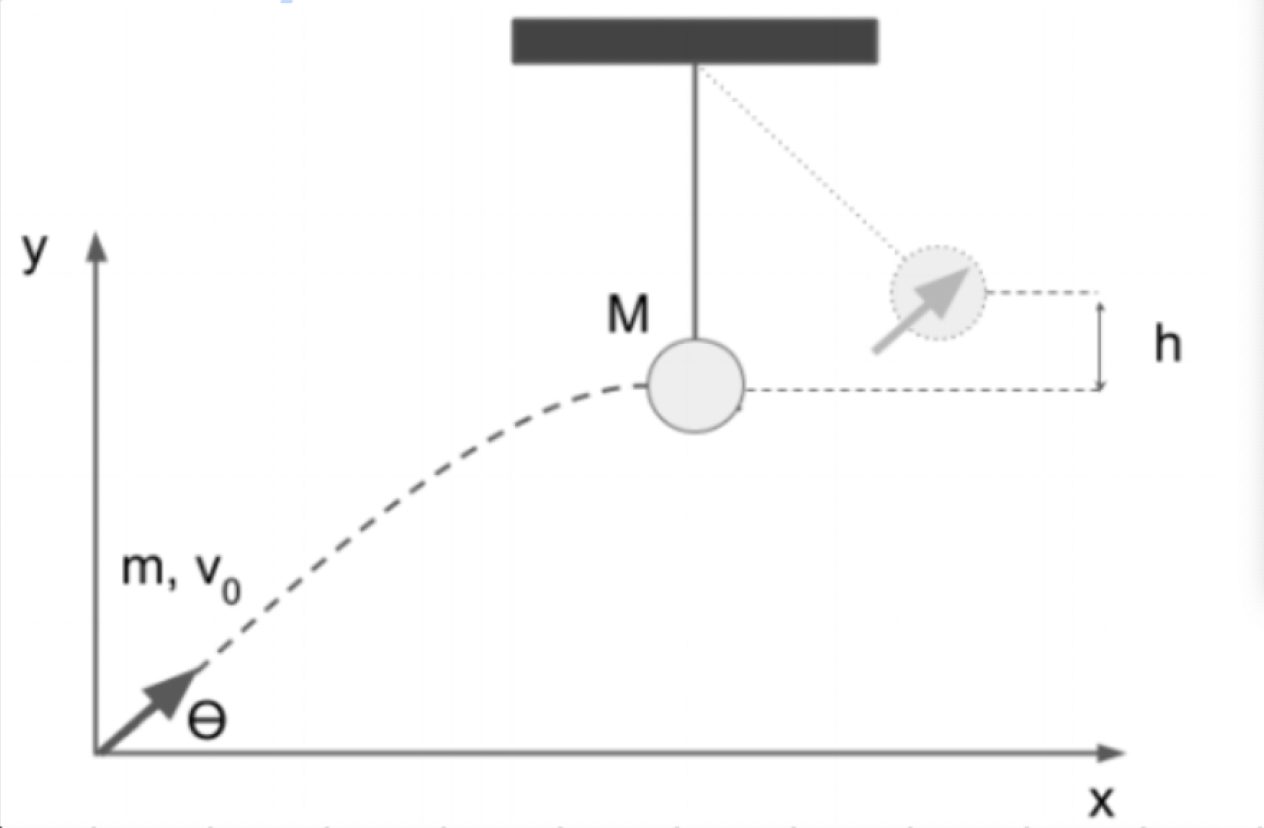
\includegraphics[width=0.5\linewidth]{Immagini/parabolicoependolo.png}
\end{figure}
\\
Soluzione:
\begin{enumerate}
    \item Calcolo della velocità orizzontale della lancia:
    \[ v_{0x} = v_0 \cos(\theta) \]
    \[ v_{0x} = 200 \cos(30^\circ) \]
    \[ v_{0x} \approx 173.2 \, \text{m/s} \]
    
    \item Conservazione della quantità di moto:
    \[ m_l v_{0x} = (m_l + M_p) v_f \]
    
    \item Calcolo della velocità finale combinata \( v_f \):
    \[ \frac{1}{2} (m_l + M_p) v_f^2 = (m_l + M_p) g h \]
    \[ \frac{1}{2} v_f^2 = g h \]
    \[ v_f = \sqrt{2 g h} \]
    \[ v_f \approx 12.9 \, \text{m/s} \]
     
    \item Soluzione per la massa del pendolo \( M_p \):
    \[ m_l v_{0x} = (m_l + M_p) v_f \]
    \[ 4.8 \cdot 173.2 = (4.8 + M_p) \cdot 12.9 \]
    \[ M_p \approx 59.7 \, \text{kg} \]
\end{enumerate}

\noindent Risultato:
\[ M_p \approx 59.7 \, \text{kg} \]
\subsection{I 2 treni}
Problema:\\
Due treni viaggiano, sulla stessa linea ferroviaria e nello stesso verso, con velocità costante v1 = 78km/h e v2 = 120km/h partendo da due stazioni distanti tra loro 200 km. Il treno 1 parte, più avanti, è quello più lento. Il treno 1 parte dalla stazione 1,2h dopo il treno 2 che segue. Dopo che i treni sono partiti si incrociano a tempo t. Trovare t. \\
\\
Soluzione:
\begin{enumerate}
    \item Condizione di incontro:
    \[ x_1(t) = x_2(t) \]
    Distanza percorsa dal treno 1 più la distanza iniziale:
    \[ 56 \, \text{km} + v_1 t = v_2 t \]
    \item Sostituzione dei valori e risoluzione per \( t \):
    \[ 56 + 78t = 120t \]
    \[ 56 = 42t \]
    \[ t = 1.33 \, \text{h} \]
\end{enumerate}

\noindent Risultato:
I treni si incontrano 1,33 ore dopo la partenza del treno 1.
\newpage
\subsection{Carrucola su piano inclinato senza attrito}
Problema:\\
Su un piano inclinato di angolo 29.42° si trova un corpo di massa m2 = 49.95kg. Tramite una fune inestensibile e una carrucola perfetta il precedente corpo e collegato a un corpo di massa m1 che si trova in caduta libera verso il suo ad altezza di 39.53m e toccherà terra dopo 4.2 secondi. Trovare m1.
\begin{figure}[ht]
    \centering
    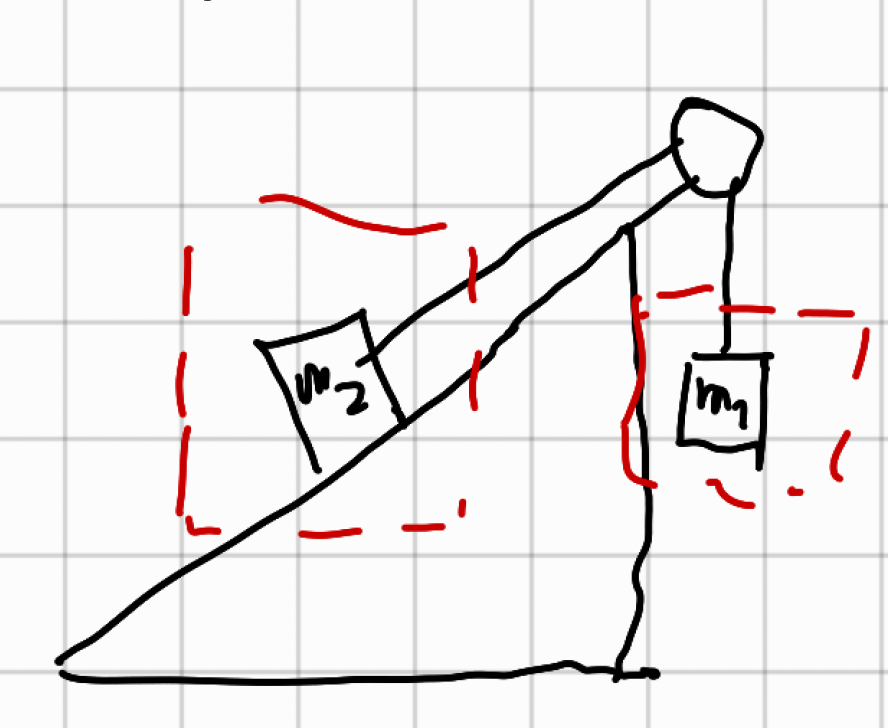
\includegraphics[width=0.5\linewidth]{Immagini/pianoinclinatocarrucola.png}
\end{figure}

Soluzione:
\begin{enumerate}
    \item Calcolo dell'accelerazione \( a \) usando il tempo di caduta:
    \[ s = s_0 + v_0t + \frac{1}{2}at^2 \]
    \[ a = \frac{2h}{t^2} \]
    \[ a = \frac{2 \cdot 39.53}{4.2^2} \]
    \[ a \approx 4.48 \, \text{m/s}^2 \]
    \item Equazioni di Newton per il sistema:
    
    Per il corpo in caduta libera \( m_1 \):
    
    \[ m_1 g - T = m_1 a \]
    
    Per il corpo sul piano inclinato \( m_2 \):
    
    \[ T - m_2 g \sin(\theta) - \mu_k m_2 g \cos(\theta) = m_2 a \]
    \item Risoluzione del sistema di equazioni:
    \[ m_1 g - m_1 a = m_2 a + m_2 g \sin(\theta) + \mu_k m_2 g \cos(\theta) \]
    \item Espressione di \( m_1 \):
    \[ m_1 = \frac{m_2 (a + g \sin(\theta) + \mu_k g \cos(\theta))}{g - a} \]
    \item Sostituzione dei valori numerici (senza coefficiente di attrito \( \mu_k \) considerato):
    
    \[ m_1 = \frac{49.95 (4.48 + 9.8 \sin(29.42^\circ))}{9.8 - 4.48} \]
    \[ \sin(29.42^\circ) \approx 0.491 \]
    \[ m_1 = \frac{49.95 (4.48 + 9.8 \cdot 0.491)}{5.32} \]
    \[ m_1 \approx 87.21 \, \text{kg} \]
\end{enumerate}

\noindent Risultato:\\
La massa del corpo \( m_1 \) è approssimativamente \( 87.21 \, \text{kg} \).
\subsection{Proiettile atterra su piano inclinato}
Problema:\\
Un proiettile viene sparato vero l'alto con angolo di alzo 23° misurato rispetto l'orizzontale e velocità iniziale v0. Dopo un tempo di 38s il proiettile incontra il piano inclinato di angolo 38° nel punto A. Trovare v0.
\begin{figure}[ht]
    \centering
    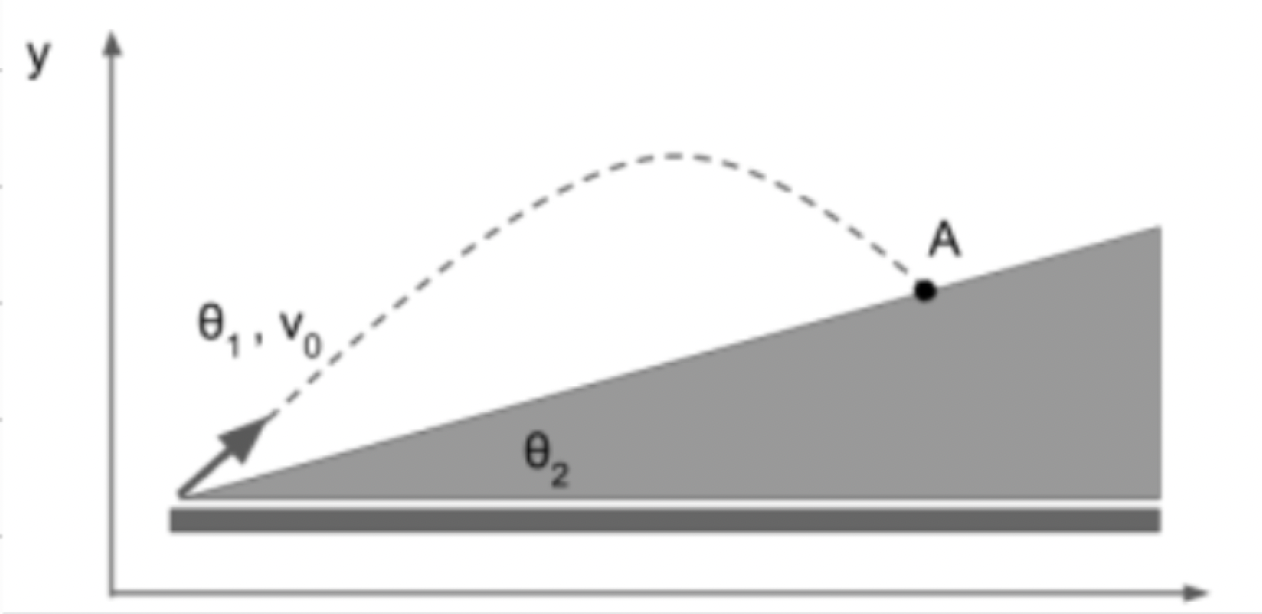
\includegraphics[width=0.5\linewidth]{Immagini/proiettinenelpiano.png}
\end{figure}

Soluzione:
\begin{enumerate}
    \item Calcolo rapporto tra X e Y 
    \[
        \begin{cases}
            X = cos \theta_2 \cdot d \\
            Y = sin \theta_2 \cdot d
        \end{cases}
    \]
    dove d rappresenta la distanza dal punto iniziale al punto A
    \[Y = X \cdot tan \theta_2\]
    \item Utilizzo questo rapporto sulla legge oraria del moto parabolico.
    \[v_0 cos(\theta_1) \cdot t \cdot tan \theta_2 = v_0 sin(\theta_1) \cdot - \frac{1}{2}gt^2\]
    \[v_0 = \frac{gt}{2(cos \theta_1 tan \theta_2 - sin \theta_1)}\]
    \[v_0 = \frac{372,78}{0,2648}\]
    \[v_0 \approx 1.47 \times 10^3 \, \text{m/s}\]
\end{enumerate}

\noindent Risultato:\\
La velocità iniziale \( v_0 \) del proiettile è approssimativamente \( 1.47 \times 10^3 \, \text{m/s} \).
\subsection{Massa sposta massa con carrucola e si toccano}
Problema:\\
Si consideri il sistema in figura. Siano M = 65 kg e m = 77 kg e a l'accelerazione del sistema. Trovare a.
\begin{figure}[ht]
    \centering
    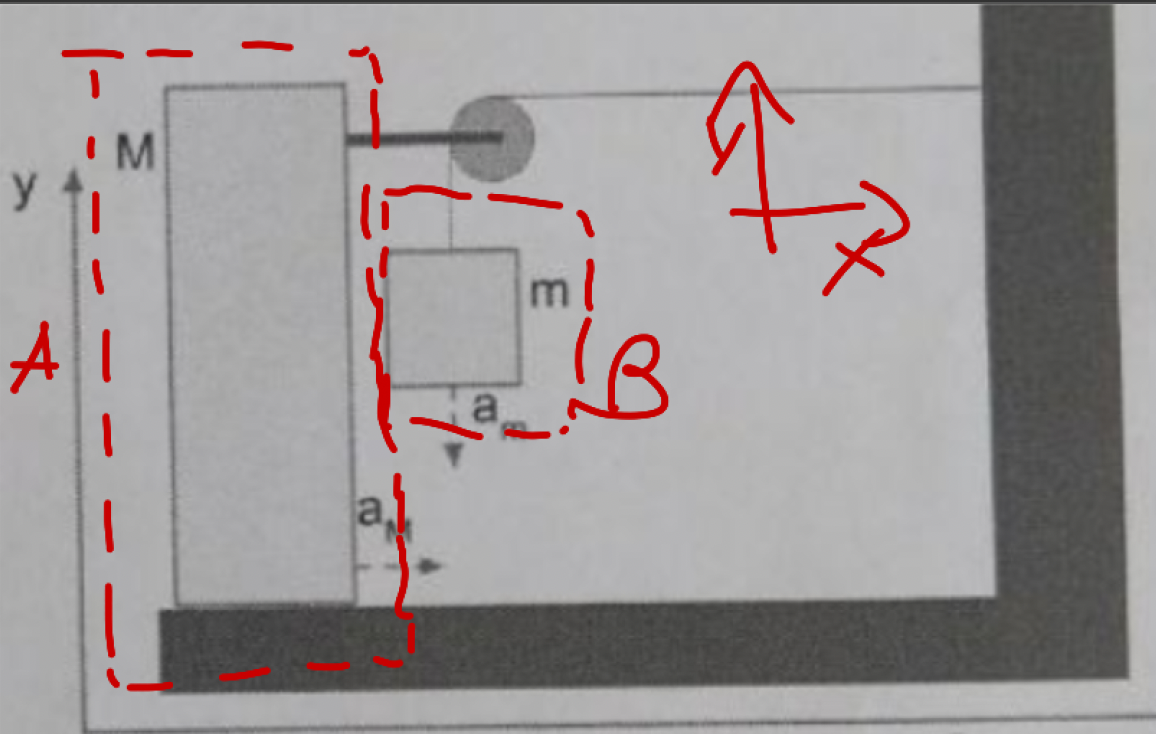
\includegraphics[width=0.5\linewidth]{Immagini/massaspostamassacarrucola.png}
\end{figure}

\noindent Soluzione:
\begin{enumerate}
    \item Equazioni dei sistema\\
    Blocco m:
    \[ m \cdot a = m \cdot g - T\]
    Blocco M:
    \[ (M + m)  a = T\]
    //\textit{\((M + m)\) perché i due blocchi si toccano, se non lo facessero allora \(M\).}
    \item Sistema di equazioni
    \[mg - ma = (M + m)a\]
    \[ a = \frac{mg}{M + 2m}\]
    \[ a = \frac{755,37}{223}\]
    \[a \approx 3,39 m/s^2\]
\end{enumerate}

\noindent Risultato:\\
L'accelerazione \(a\) del sistema è \(3,39 m/s^2\)
\subsection{Appeso a due molle}
Problema:\\
Un corpo di massa m trascurabile è appeso con due molle di lunghezza a riposo nulla e costante elastica k. Al corpo viene applicata una forza di 99N diretta verso il basso. Nella condizione di equilibrio le molle individuano tra esse un angolo di 38° e si allungano di 12 m. Trovare k.
\begin{figure}[ht]
    \centering
    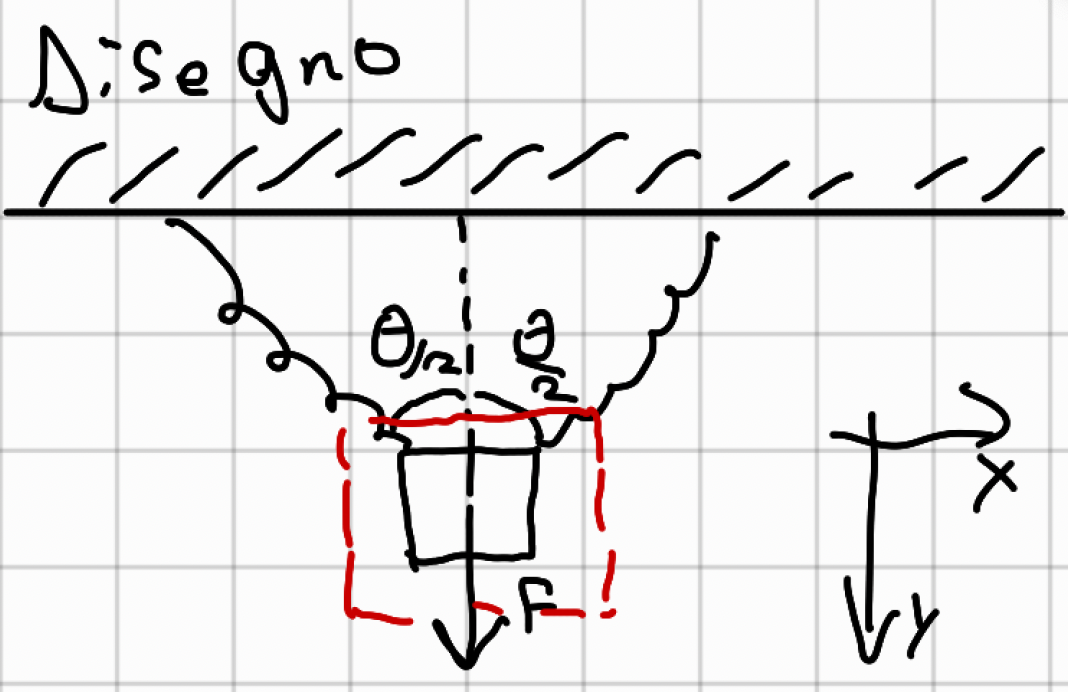
\includegraphics[width=0.5\linewidth]{Immagini/appesotraduemolle.png}
\end{figure}

\noindent Soluzione:
\begin{enumerate}
    \item Cerco la F Perpendicolare delle molle
    \[ F_\perp = F_{e1} \cdot cos \theta_1\]
    dove
    \[\theta = \theta_1 + \theta_2\]
    \item Metto in relazione le forze che spingono in basso con quelle opposte
    \[F + F_p = F_{\perp1} + F_{\perp2}\]
    essendo la forza peso trascurabile da testo allora
    \[2(k\cdot \Delta x \cdot cos\theta_1) = F\]
    \[k = \frac{F}{2(\Delta x \cdot cos\theta_1)}\]
    \[k =  \frac{99}{22,8}\]
    \[k \approx 4,34 \text{N/m}\]
\end{enumerate}

\noindent Risultato:\\
La costante \(k\) delle molle misura \(4,34 \text{N/m}\)
\newpage
\subsection{Oggetto scivola dopo piano inclinato}
Problema:\\
Un corpo di massa m fermo inizia a scivolare su un piano inclinato alto 51 m. Alla base del piano, il corpo inizia a muoversi su un piano orizzontale con coefficiente di attrito dinamico di 0.55 e si ferma dopo l metri. Trovare \(\Delta\)l
\begin{figure}[ht]
    \centering
    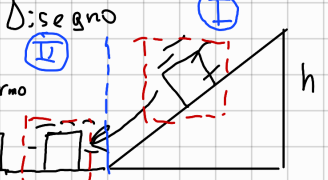
\includegraphics[width=0.5\linewidth]{Immagini/oggettoscivolapianoinclinatoesiferma.png}
\end{figure}

\noindent Soluzione:
\begin{enumerate}
    \item Utilizzo la conservazione dell'energia per trova la velocità iniziale
    \[U_0 = K\]
    \[mgh = \frac{1}{2}mv^2\]
    \[ v = \sqrt{2gh}\]
    \item Cerco le forze che vengono applicate all'oggetto
    \[ F = F_a = F_p\cdot \mu_d\]
    \[ ma = mg\cdot \mu_d\]
    \[ a = g\cdot \mu_d\]
    \item Trovo lo spazio percorso dalla decelerazione
    \[ s=\frac{V_0^2}{2a}\]
    \[ s = \frac{2gh}{2g\cdot \mu_d}\]
    \[ s = \frac{h}{\mu_d}\]
    \[ s \approx 92,72 \text{m}\]
\end{enumerate}

\noindent Risultato:\\
L'oggetto si ferma dopo 92,72 m
\newpage
\subsection{Proiettile che sposta costante}
Problema:\\
Su Titano (gTitano = \(1.352 m/s^2\) l'esercito di Thanos spara ad Hulk di massa 680 kg una raffica di proiettili di massa 3,4 kg e velocità 26 m/s con frequenza di 8.8 Hz. I proiettili non scalfiscono la dura pelle di Hulk e tornano indietro, ma fanno scivolare indietro l'uomo verde a velocità costante. Il coefficiente d'attrito dinamico tra i piedi di Hulk e la superficie di Titano è \(\mu_d\). Trovare \(\mu_d\).
\begin{figure}[ht]
    \centering
    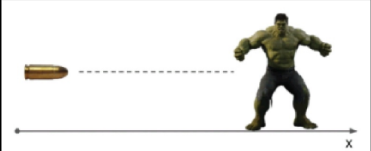
\includegraphics[width=0.5\linewidth]{Immagini/Hulkscivola.png}
\end{figure}

\noindent Soluzione:
\begin{enumerate}
    \item Trovo il periodo dei proiettili
    \[T = \frac{1}{f}\]
    \item Metto in relazione le forze su Hulk
    \[ F_a = F_{proiettile}\]
    \item Trovo la forza del proiettile\\
    Essendo che la risultante delle forze è 0 applicato il Principio di conversazione del moto
    \[m_{p}v_p = - m_pv_p\]
    \[2m_pv_p = 0\]
    \[F_{proiettile} = \frac{2m_pv_p}{T}\]
    \item Risolvo l'equazione per \(\mu\)
    \[m_H \cdot g_T \cdot \mu_d = \frac{2m_pv_p}{T}\]
    \[\mu_d = \frac{2m_pv_p}{T \cdot m_H \dot g_T}\]
    \[\mu_d \approx 1.69\]
\end{enumerate}

\noindent Risultato:\\
L'attrito tra Hulk e la superficie di Titano è 1,74.
\end{document}
